\documentclass{beamer}

\usepackage[T1]{fontenc}
\usepackage[utf8]{inputenc}
\usepackage[slovene]{babel}

\usepackage{palatino}
\usefonttheme{serif}

\usepackage{amsfonts}
\usepackage{amsmath,amsthm}

\usepackage{tikz}
\usepackage{pgfplots}
\usetikzlibrary{intersections}
\usepgfplotslibrary{fillbetween}
\pgfplotsset{compat=newest}

\usetheme{CambridgeUS}
\usecolortheme{dolphin}
\setbeamertemplate{navigation symbols}{}
%\setbeamertemplate{footline}[frame number]{}

\linespread{1.2}

\newcommand{\N}{\mathbb{N}}
\newcommand{\Z}{\mathbb{Z}}
\newcommand{\Q}{\mathbb{Q}}
\newcommand{\R}{\mathbb{R}}
\newcommand{\C}{\mathbb{C}}

\newtheorem{izrek}{Izrek}
\newtheorem{trditev}[izrek]{Trditev}
\newtheorem{posledica}[izrek]{Posledica}
\newtheorem{definicija}[izrek]{Definicija}
\newtheorem{naloga}[izrek]{Naloga}
\newtheorem{resitev}[izrek]{Naloga}

\begin{document}

\title{20. naloga}
\author{Janez Podlogar}
\date{9. 5. 2022}

\begin{frame}
    \titlepage
\end{frame}

\begin{frame}
    \frametitle{Navodilo naloge}
Streljamo v tarčo kvadratne oblike z robom $a$. Predpostavimo, da vsak zadetek zadene
tarčo in da je točka zadetka porazdeljena enakomerno po tarči. Izračunaj verjetnost, da
bo naš strel zadel bližje središču tarče kot njenemu robu.
\end{frame}

\begin{frame}
    \frametitle{Rešitev}
\begin{itemize}
    \item Naj bo $T_a = \left[ -\frac{a}{2} , \frac{a}{2}\right]\times\left[-\frac{a}{2},\frac{a}{2}\right]$ tarča
    \item Z $S_a$ označimo množico vseh točk, ki so bližje središču tarče kot robu tarče
\end{itemize}
Zanima nas verjetnost, da je točka vsebovana v množici $S_a$
\begin{align*}
    P\big((x,y) \in B\big)
    &= \frac{pl(S_a)}{pl(T_a)} \\[1em]
    &= \frac{1}{a^2} \iint\limits_{S_a} 1 \, \mathrm{d}x\mathrm{d}y
\end{align*}
\end{frame}

\begin{frame}
    \frametitle{Rešitev}
    \begin{figure}[h!]
        \centering
        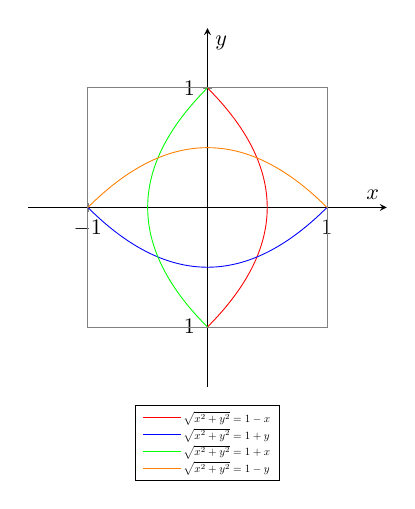
\begin{tikzpicture}[scale=0.8]
            \begin{axis}[
                axis equal image,
                %hide axis,
                axis lines=center,
                xlabel={$x$}, xmin=-1.5, xmax=1.5,
                ylabel={$y$}, ymin=-1.5, ymax=1.5,
                %extra x ticks={-1,1},
                %extra y ticks={-1,1},
                %extra tick style={grid=major},
                legend style={at={(0.5,-0.05)},anchor=north, legend cell align=left, nodes={scale=0.5, transform shape}},
                legend entries={$\sqrt{x^2+y^2}=1-x$, $\sqrt{x^2+y^2}=1+y$, $\sqrt{x^2+y^2}=1+x$, $\sqrt{x^2+y^2}=1-y$}
                ]
                \draw[gray, thin] (-1,-1) rectangle (1,1);
                \addplot[red, domain=-1:1, samples=100]({(1-x^2)/2},{x});
                \addplot[blue, domain=-1:1, samples=100]({x},{((x^2-1)/2});
                \addplot[green, domain=-1:1, samples=100]({(x^2-1)/2},{x});
                \addplot[orange ,domain=-1:1, samples=100]({x},{(1-x^2)/2});
            \end{axis}
        \end{tikzpicture}
        \caption{Roboni pogoji pri $a=2$}
    \end{figure}
\end{frame}

\begin{frame}
    \frametitle{Rešitev}
    \begin{figure}[!ht]
        \centering
        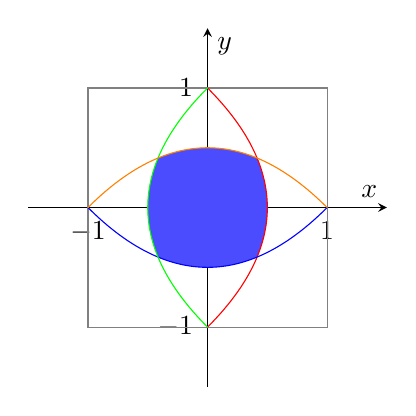
\begin{tikzpicture}[scale=0.8]
            \begin{axis}[
                axis equal image,
                %hide axis,
                axis lines=center,
                xlabel={$x$}, xmin=-1.5, xmax=1.5,
                ylabel={$y$}, ymin=-1.5, ymax=1.5,
                %extra x ticks={-1,1},
                %extra y ticks={-1,1},
                %extra tick style={grid=major},
                %legend style={at={(0.63,-0.05)},anchor=north, legend cell align=left, nodes={scale=0.5, transform shape}},
                %legend entries={$\sqrt{x^2+y^2}=1-x$, $\sqrt{x^2+y^2}=1+y$, $\sqrt{x^2+y^2}=1+x$, $\sqrt{x^2+y^2}=1-y$}
                ]
                \draw[gray, thin] (-1,-1) rectangle (1,1);
                \addplot[red, domain=-1:1, samples=100]({(1-x^2)/2},{x});
                \addplot[blue, domain=-1:1, samples=100]({x},{((x^2-1)/2});
                \addplot[green, domain=-1:1, samples=100]({(x^2-1)/2},{x});
                \addplot[orange ,domain=-1:1, samples=100]({x},{(1-x^2)/2});
                \addplot[forget plot, draw=none, domain=-0.414:0.414, samples=100, name path=A]({(1-x^2)/2},{x});
                \addplot[forget plot, draw=none, domain=-0.414:0.414, samples=100, name path=B]({x},{((x^2-1)/2});
                \addplot[forget plot, draw=none, domain=-0.414:0.414, samples=100, name path=C]({(x^2-1)/2},{x});
                \addplot[forget plot, draw=none, domain=-0.414:0.414, samples=100, name path=D]({x},{(1-x^2)/2});
                \addplot[blue!70] fill between[of=A and C];
                \addplot[blue!70] fill between[of=B and D];
            \end{axis}
        \end{tikzpicture}
        \caption{Integral $\iint\limits_{S_2} 1 \, \mathrm{d}x\mathrm{d}y$}
    \end{figure}
\end{frame}

\begin{frame}
    \frametitle{Rešitev}
Ploščino najlažje izračunamo tako, da opazimo simetrijo rotacij in simetrijo zrcaljenja.
Izračunali bomo ploščino le enega izmed osmih trikotnikov
\begin{figure}[!ht]
    \centering
    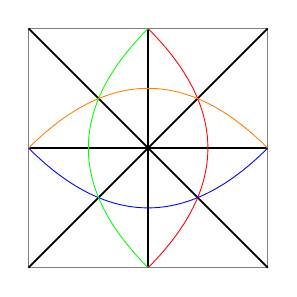
\begin{tikzpicture}[scale=0.8]
        \begin{axis}[
            axis equal image,
            hide axis,
            axis lines=center,
            xlabel={$x$}, xmin=-1.5, xmax=1.5,
            ylabel={$y$}, ymin=-1.5, ymax=1.5,
            %extra x ticks={-1,1},
            %extra y ticks={-1,1},
            %extra tick style={grid=major},
            legend style={at={(0.5,-0.07)},anchor=north, legend cell align=left, nodes={scale=0.5, transform shape}},
            %legend entries={$\sqrt{x^2+y^2}=1-x$, $\sqrt{x^2+y^2}=1+y$, $\sqrt{x^2+y^2}=1-x$, $\sqrt{x^2+y^2}=1+x$}
            ]
            \draw[gray, thin] (-1,-1) rectangle (1,1);
            \addplot[black, thick, domain=-1:1, samples=100]{x};
            \addplot[black, thick, domain=-1:1, samples=100]{-x};
            \addplot[black, thick, domain=-1:1, samples=100]{0};
            \addplot[black, thick, domain=-1:1, samples=100]({0},{x});
            \addplot[red, domain=-1:1, samples=100]({(1-x^2)/2},{x});
            \addplot[blue, domain=-1:1, samples=100]({x},{((x^2-1)/2});
            \addplot[green, domain=-1:1, samples=100]({(x^2-1)/2},{x});
            \addplot[orange ,domain=-1:1, samples=100]({x},{(1-x^2)/2});
        \end{axis}
    \end{tikzpicture}
    \caption{Simetrije}
\end{figure}
\end{frame}

\begin{frame}
    \frametitle{Rešitev}
    \begin{figure}[!ht]
        \centering
        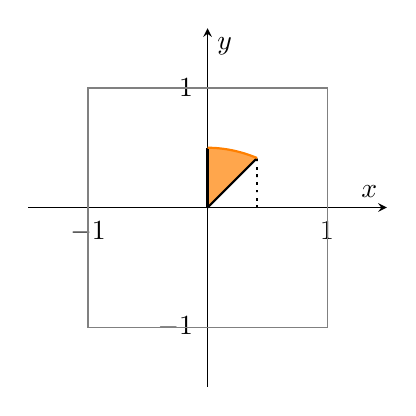
\begin{tikzpicture}[scale=0.8]
            \begin{axis}[
                axis equal image,
                %hide axis,
                axis lines=center,
                xlabel={$x$}, xmin=-1.5, xmax=1.5,
                ylabel={$y$}, ymin=-1.5, ymax=1.5,
                %extra x ticks={-1,1},
                %extra y ticks={-1,1},
                %extra tick style={grid=major},
                %legend style={at={(0.5,-0.07)},anchor=north, legend cell align=left, nodes={scale=0.5, transform shape}},
                %legend entries={$\sqrt{x^2+y^2}=1-x$, $\sqrt{x^2+y^2}=1+y$, $\sqrt{x^2+y^2}=1-x$, $\sqrt{x^2+y^2}=1+x$}
                ]
                \draw[gray, thin] (-1,-1) rectangle (1,1);
                \addplot[black, thick, domain=0:0.414, samples=100, name path=D]{x};
                \addplot[black, thick, domain=0:0.5, samples=100]({0},{x});
                \addplot[black, thick, dotted, domain=0:0.414, samples=100]({0.414},{x});
                \addplot[orange, thick, domain=0:0.414, samples=100, name path=B]({x},{((1-x^2)/2});
                \addplot[orange!70] fill between[of=B and D];
            \end{axis}
        \end{tikzpicture}
        \caption{Osmina ploščine pri $a=2$}
    \end{figure}
\end{frame}

\begin{frame}
    \frametitle{Rešitev}
\begin{itemize}
\item Funkcijo $|(x,y)| < \frac{a}{2} - y$, ki opisuje vse točke, ki so bližje središču tarče kot
zgornjemu robu tarče preoblikujemo v 
\begin{equation*}
    y = \frac{a}{4} - \frac{x^2}{a}
\end{equation*}

\item Poiščemo njeno presečišče z funkcijo $y = x$. Ko rešimo kvadratno enačbo,
dobimo za ustrzno presečišče
\begin{equation*}
    x=\frac{a(\sqrt{2}-1)}{2}
\end{equation*}
\end{itemize}
\end{frame}

\begin{frame}
    \frametitle{Rešitev}
\begin{itemize}
\item Izračunajmo ploščino oranžnega območja
\begin{align*}
    \int_{0}^{\frac{a(\sqrt{2}-1)}{2}} \frac{a}{4} - \frac{x^2}{a} \, \mathrm{d}x - \frac{1}{2}(\frac{a(\sqrt{2}-1)}{2})^2
    &= \frac{a^2(4-2\sqrt{2})}{24} - \frac{a^2(3-2\sqrt{2})}{8} \\
    &= \frac{a^2(4\sqrt{2}-5)}{24}
\end{align*}
\item Ploščino celotnega območja dobimo tako, da pomnožimo zgorjno ploščino z $8$
\item Verjetnost, da strel zadane bližje središču tarče kot njenemu robu je enaka
\begin{equation*}
    P\big((x,y) \in S_a\big) = \frac{4\sqrt{2}-5}{3} \approx 0.218951416
\end{equation*}
\end{itemize}
\end{frame}

\begin{frame}
    \frametitle{Simulacija}
    Tabela prikazuje rezulate simulacije ter njihovo absolutno in relativno
    napako na devet decimalk natančno
    \begin{table}[!ht]
        \footnotesize
        \begin{tabular}{|c|l|l|l|}
        \hline
        \textbf{Število točk} & \textbf{Vrednost simulacije} & \textbf{Absolutna napaka} & \textbf{Relativna napaka} \\ \hline
        $10^3$                & 0.229                        & 0.010048584               & 0.045894127               \\ \hline
        $10^4$                & 0.2247                       & 0.005748584               & 0.026255067               \\ \hline
        $10^5$                & 0.21732                      & 0.001631416               & 0.007451041               \\ \hline
        $10^6$                & 0.218713                     & 0.000238416               & 0.001088899               \\ \hline
        $10^7$                & 0.2187818                    & 0.000169616               & 0.000774674               \\ \hline
        $10^8$                & 0.21904325                   & 0.000091834               & 0.000419426               \\ \hline
        \end{tabular}
        \end{table}
\end{frame}

\end{document}
